\documentclass[../laporan]{subfiles}

\begin{document}

\section{Hasil dan Pembahasan}

\subsection{Percobaan Pertama}

Pada percobaan pertama,dibuat diagram blok yang membandingkan respon orde sistem dibuat pada simulink sebagaimana ditunjukkan pada Gambar \ref{soal_1_a}.

\begin{figure}[H]
    \centering
    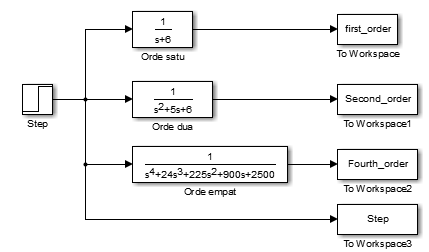
\includegraphics[width = 0.5\textwidth]{figure/soal_1_a.png}
    \caption{Diagram blok perbandingan orde sistem menggunakan simulink}
    \label{soal_1_a}
\end{figure}

Hasil dari simulasi menunjukkan perbedaan respon sistem ditunjukkan pada Gambar \ref{hasil_1_a}. Hasil simulasi menunjukkan ada perbedaan antara respon sistem orde satu, orde dua, dan orde empat. Respon dari sistem orde satu dan dua tidak menunjukkan adanya overshoot. Overshoot merupakan kondisi output sistem yang melebihi batas kondisi steady-state. Sehingga, dapat disimpulkan dari pengamatan performansi respon bahwa sistem dengan orde satu dan dua pada simulasi ini lebih stabil dibandingkan dengan sistem orde empat. Dari hasil simulasi ini juga terlihat bahwa sistem orde satu memiliki respon terhadap input yang lebih cepat daripada sistem orde dua karena berdasarkan pengamatan hasil simulasi sistem memiliki rise time yang lebih cepat, hal ini dapat dilihat dari garis output sistem satu yang lebi cepat menyentuh keadaan steady state dibanding sistem orde dua.

\begin{figure}[H]
    \centering
    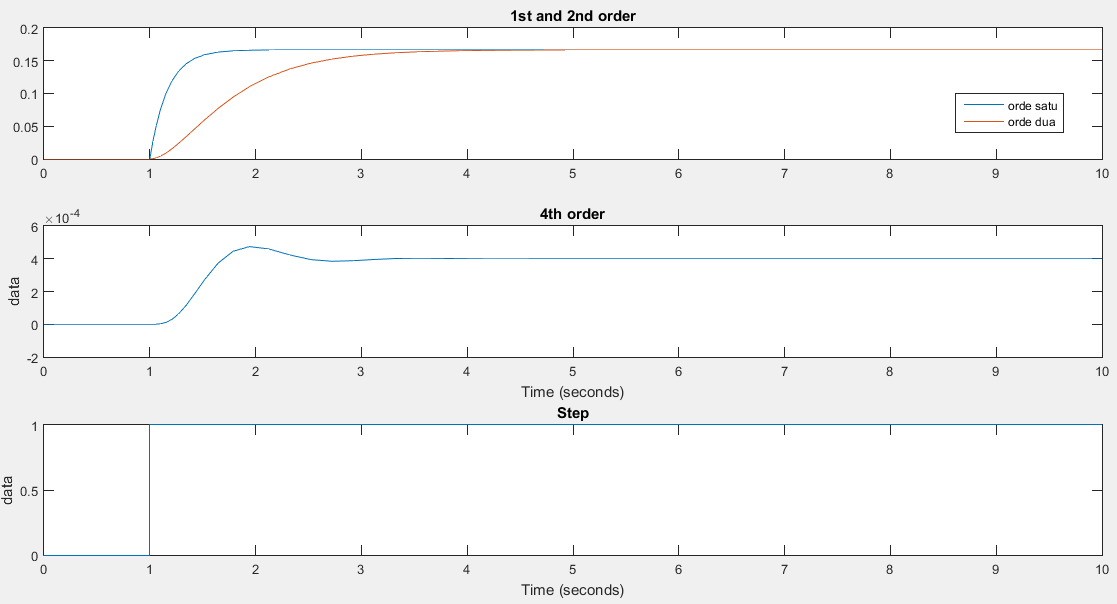
\includegraphics[width = 0.7\textwidth]{figure/hasil_1_a.png}
    \caption{Plot hasil perbandingan orde sistem}
    \label{hasil_1_a}
\end{figure}

\subsection{Percobaan kedua}

Pada percobaan kedua, dibuat diagram blok yang membandingkan keluaran sistem dengan variasi nilai rasio redaman ($\xi$) pada masing-masing sistem. Diagram blok simulasi ditunjukkan pada Gambar \ref{soal_1_b}.

\begin{figure}[H]
    \centering
    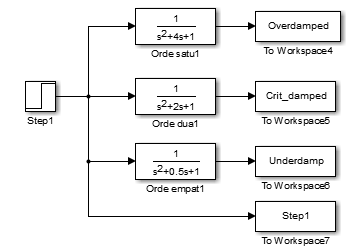
\includegraphics[width = 0.6\textwidth]{figure/soal_1_b.png}
    \caption{Diagram blok perbandingan sistem dengan variasi nilai rasio redaman}
    \label{soal_1_b}
\end{figure}

Hasil simulasi dari percobaan kedua menunjukkan perbedaan respon sistem seperti yang ditunjukkan pada Gambar \ref{hasil_1_b}. Hasil ini sesuai dengan analisis mamematis sistem nilai rasio redaman sistem. Dengan persamaan matematis sistem sebagai berikut,

\begin{equation}
    \frac{C_{(s)}}{R_{(s)}} = K\frac{\omega_n^2}{s^2+2\xi\omega_n s+\omega_{n}^2}
    \label{persamaan_sistem_orde_dua}
\end{equation}

Dari bentuk matematis sistem orde dua yang ditunjukkan pada persamaan \eqref{persamaan_sistem_orde_dua}. Dapat dilakukan analisis pada masing-masing sistem sebagai berikut,

\begin{equation*}
\label{persamaan_orde_dua}
    \begin{split}
        \text{Analisis pada sistem satu,}\\
        4 &= 2\xi\omega_ns \\[5pt]
        4 &= 2\xi \\[5pt]
        2 &= \xi \Rightarrow \text{sistem mengalami overdamped} \\[5pt]
        \text{Analisis pada sistem dua,}\\
        2 &= 2\xi\omega_ns \\[5pt]
        2 &= 2\xi \\[5pt]
        1 &= \xi \Rightarrow \text{sistem mengalami critically damped} \\[5pt]
        \text{Analisis pada sistem tiga,}\\
        0.5 &= 2\xi\omega_ns \\[5pt]
        0.5 &= 2\xi \\[5pt]
        0.25 &= \xi \Rightarrow \text{sistem mengalami underdamped}
    \end{split}
\end{equation*}

Hasil analisis matematis cocok dengan hasil simulasi yang memperlihatkan bahwa terdapat tiga sistem yang berbeda pada grafik hasil simulasi. Terdapat satu sistem yang mengalami overdamped, ada satu sistem yang mengalami critically damped, dan ada satu sistem yang mengalami underdamped. sistem yang mengalami overdamped memiliki garis keluaran yang berada dibawah garis masukan step, sistem yang mengalami critically damped memiliki garis keluaran yang berhimpitan dengan garis masukan step, dan sistem yang mengalami underdamped memiliki garis keluaran yang melampaui garis masukan step.

\begin{figure}[H]
    \centering
    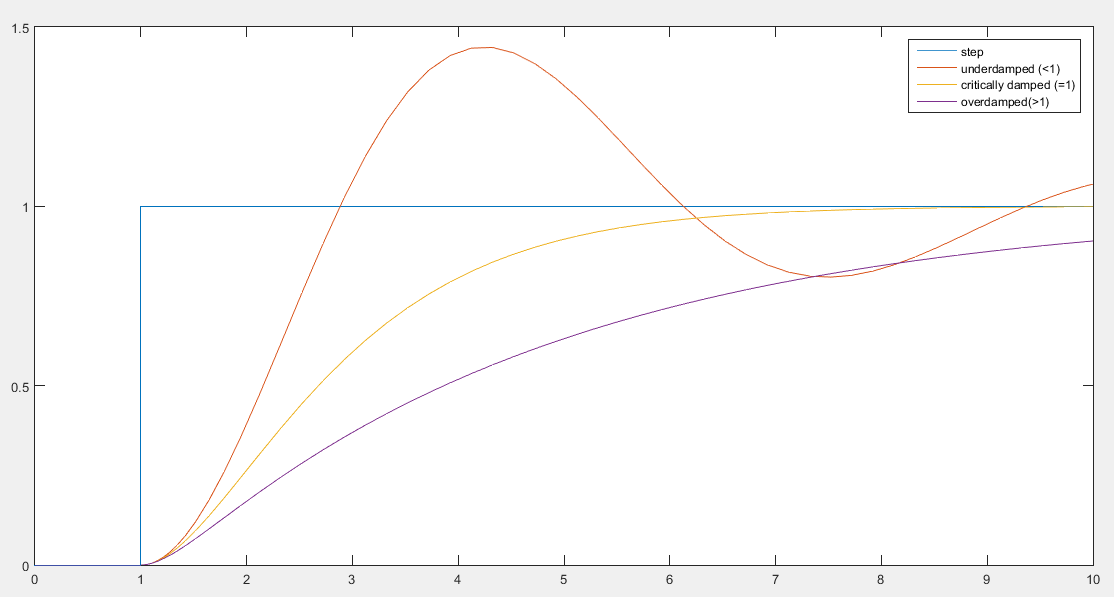
\includegraphics[width = 0.8\textwidth]{figure/hasil_1_b.png}
    \caption{Hasil simulasi perbandingan pengaruh rasio redaman}
    \label{hasil_1_b}
\end{figure}

\subsection{Analisis Sistem Orde Satu}

Dilakukan analisis matematis terhadap sebuah sistem dengan persamaan sebagai berikut,

\begin{equation*}
    \frac{Y_{(s)}}{X_{(s)}} = \frac{6}{s+10}
\end{equation*}

Dari persamaan tersebut dianalisis untuk menemukan,

\begin{itemize}
    \item time constant ($\tau$)
    \item waktu bangkit (rise time)
    \item waktu endap (setling time)
    \item waktu tunda (delay time)
    \item plot respon sistem
\end{itemize}

analisis dari sistem orde satu sebagai berikut,

\subsubsection{time constant ($\tau$)}

Nilai dari time constant dapat dicari dengan persamaan berikut,

\begin{equation}
\begin{split}
    \frac{Y_{(s)}}{X_{(s)}} &= \frac{1}{\tau s+1} \\[5pt]
    \frac{Y_{(s)}}{X_{(s)}} &= \frac{6}{s+10}\\[5pt]
    \frac{Y_{(s)}}{X_{(s)}} &= \frac{\frac{6}{10}}{\frac{1}{10}s+\frac{10}{10}}\\[5pt]
    \frac{Y_{(s)}}{X_{(s)}} &= \frac{0.6}{0.1s+1} \Rightarrow \tau = 0.1
\end{split}
\end{equation}

Dari persamaan diatas, dapat diketahui bahwa nilai time constant ($ \tau $) pada sistem adalah $ 0.1 $.



\subsubsection{Waktu Bangkit (T_r)}

Waktu bangkit pada sistem orde satu dapat diperoleh melalui persamaan berikut,

\begin{equation}
    \begin{split}
        T_r &= \tau\ln{19} \Rightarrow T_r(5\% - 95\%) \\[5pt]
        T_r &= 0.1[2.944] \\[5pt]
        T_r &= 0.2944
    \end{split}
\end{equation}

\begin{equation}
    \begin{split}
        T_r &= \tau\ln{9} \Rightarrow T_r(10\% - 90\%) \\[5pt]
        T_r &= 0.1[2.197] \\[5pt]
        T_r &= 0.2197
    \end{split}
\end{equation}

\subsubsection{Waktu Endap (T_s)}

Waktu endap pada sistem orde satu dapat diperoleh melalui persamaan berikut,
\begin{equation}
    \begin{split}
        T_s(\pm5\%) &= 3\tau \\[5pt]
        T_s(\pm5\%) &= 3[0.1] \Rightarrow T_s(\pm5\%) = 0.3 \text{ detik}
    \end{split}
\end{equation}
\begin{equation}
    \begin{split}
        T_s(\pm2\%) &= 4\tau \\[5pt]
        T_s(\pm2\%) &= 4[0.1] \Rightarrow T_s(\pm2\%) = 0.4 \text{ detik}
    \end{split}
\end{equation}
\begin{equation}
    \begin{split}
        T_s(\pm0.5\%) &= 5\tau \\[5pt]
        T_s(\pm0.5\%) &= 5[0.1] \Rightarrow T_s(\pm0.5\%) = 0.5 \text{ detik}
    \end{split}
\end{equation}

Dari persamaan diatas didapatkan masing-masing nilai waktu endap adalah $T_s(\pm5\%) = 0.3$ detik, $T_s(\pm2\%) = 0.4$ detik, $T_s(\pm0.5\%) = 0.5$ detik.

\subsubsection{Waktu Tunda (T_d)}

Waktu tunda dapat hitung melalui persamaan berikut,

\begin{equation}
    \begin{split}
        T_d &= \tau\ln{2} \\[5pt]
        T_d &= 0.1[0.693] \\[5pt]
        T_d &= 0.0693 \text{ detik}
    \end{split}
\end{equation}

Dari hasil persamaan diatas diketahui sistem memiliki waktu tunda sebesar $T_d = 0.0693$ detik.

\subsubsection{Plot sistem orde satu}

\begin{figure}[H]
    \centering
    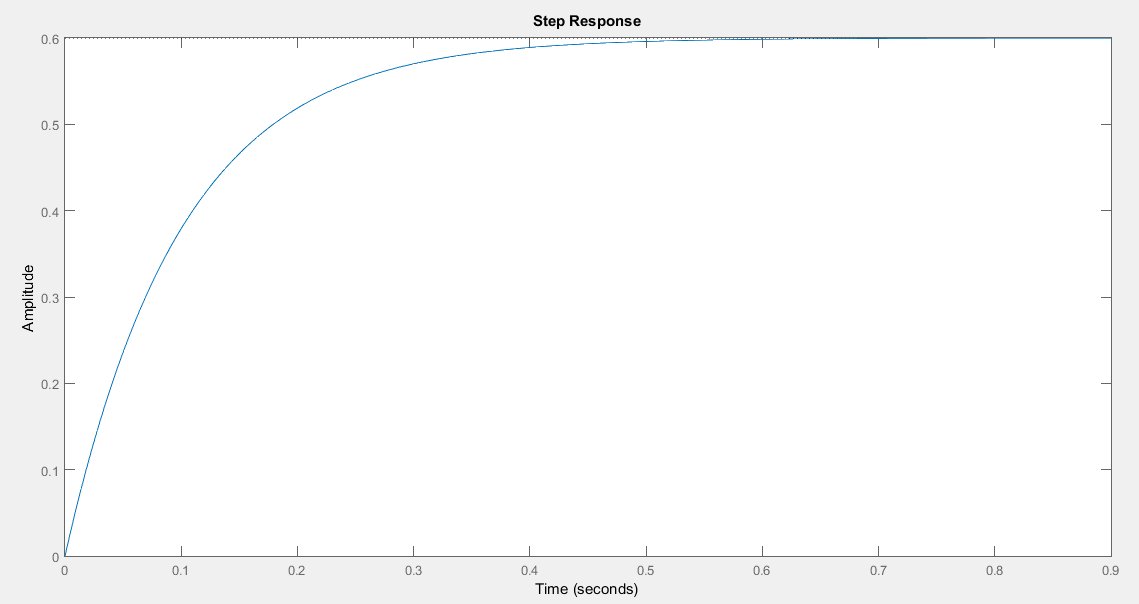
\includegraphics[width = 0.8\textwidth]{figure/plot_orde_satu.png}
    \caption{Hasil plot sistem orde satu}
\end{figure}

\subsection{Analisis Sistem Orde Dua}

Dilakukan analisis matematis terhadap sebuah sistem dengan persamaan sebagai berikut,

\begin{equation*}
    \frac{Y_{(s)}}{X_{(s)}} = \frac{1500}{s^2+10s+1500}
\end{equation*}

Dari persamaan tersebut dianalisis untuk menemukan,

\begin{itemize}
    \item Nisbah redaman ($\xi$)
    \item time constant ($\tau$)
    \item maksimum overshoot ($\%MP$)
    \item waktu bangkit (rise time)
    \item waktu endap (setling time)
    \item waktu tunda (delay time)
    \item plot respon sistem dan mengamati bentuk plot
\end{itemize}

\subsubsection{Nisbah Redaman}

Nisbah redaman dapat dihitung dengan persamaan berikut,

\begin{equation}
    \begin{split}
        \omega_n &= \sqrt{1500}\\[5pt]
        \omega_n &= 38.729\\[10pt]
        \xi &= \frac{10}{2\omega_n} \\[5pt]
        \xi &= \frac{10}{2[38.729]} \Rightarrow \xi = 0.129 \\[5pt]
    \end{split}
\end{equation}

\subsubsection{Time Constant}

Nilai time constant dapat dihitung dengan persamaan berikut,

\begin{equation}
    \begin{split}
        \tau &= \frac{1}{\xi\omega_n} = \frac{1}{0.129[38.729]} \\[5pt]
        \tau &= 0.2
    \end{split}
\end{equation}

\subsubsection{Maksimum Overshoot}

Nilai maksimum overshoot dapat dihitung dengan persamaan sebagai berikut,

\begin{equation}
    \begin{split}
        \%MP &= \exp{-\frac{\pi\xi}{\sqrt{1 - \xi^2}}}*100 \\[5pt]
        \%MP &= \exp{-\frac{\pi[38.729]}{\sqrt{1 - 38.729^2}}}*100 \\[5pt]
        \%MP &= 66.43 \%
    \end{split}
\end{equation}

\subsubsection{Waktu Bangkit}

Nilai waktu bangkit dapat dicari dengan persamaan berikut,

\begin{equation}
    \begin{split}
        T_r &= \frac{1}{\omega_n\sqrt{1-\xi^2}}[\pi-\arctan\frac{\sqrt{1-\xi^2}}{\xi}] \\[5pt]
        T_r &= \frac{1}{[38.729]\sqrt{1-0.129^2}}[\pi-\arctan\frac{\sqrt{1-0.129^2}}{0.129}] \\[5pt]
        T_r &= 0.0811 \text{ detik}
    \end{split}
\end{equation}

\subsubsection{Waktu Endap}

Nilai waktu endap dapat dicari dengan persamaan berikut,

\begin{equation}
    \begin{split}
        T_s(\pm5\%) &= 3\tau \Rightarrow T_s(\pm5\%) = 3[0.2] = 0.6 \text{ detik} \\[5pt]
        T_s(\pm2\%) &= 4\tau \Rightarrow T_s(\pm5\%) = 4[0.2] = 0.8 \text{ detik}\\[5pt]
        T_s(\pm0.5\%) &= 5\tau \Rightarrow T_s(\pm5\%) = 5[0.2] = 1 \text{ detik}
    \end{split}
\end{equation}

\subsubsection{Waktu Tunda}

Nilai waktu tunda pada sistem dapat dihitung dari persamaan berikut,

\begin{equation}
    \begin{split}
        T_d = 0.742\tau \Rightarrow T_d = 0.742[0.2] = 0.1484 \text{ detik}
    \end{split}
\end{equation}

\subsubsection{Plot respon sistem orde dua}

Dari grafik yang ditunjukkan dibawah dapat terlihat sistem mengalami overshoot, osilasi dan dalam keadaan underdamped, karena nilai$ \xi = 0.129 $

\begin{figure}[H]
    \centering
    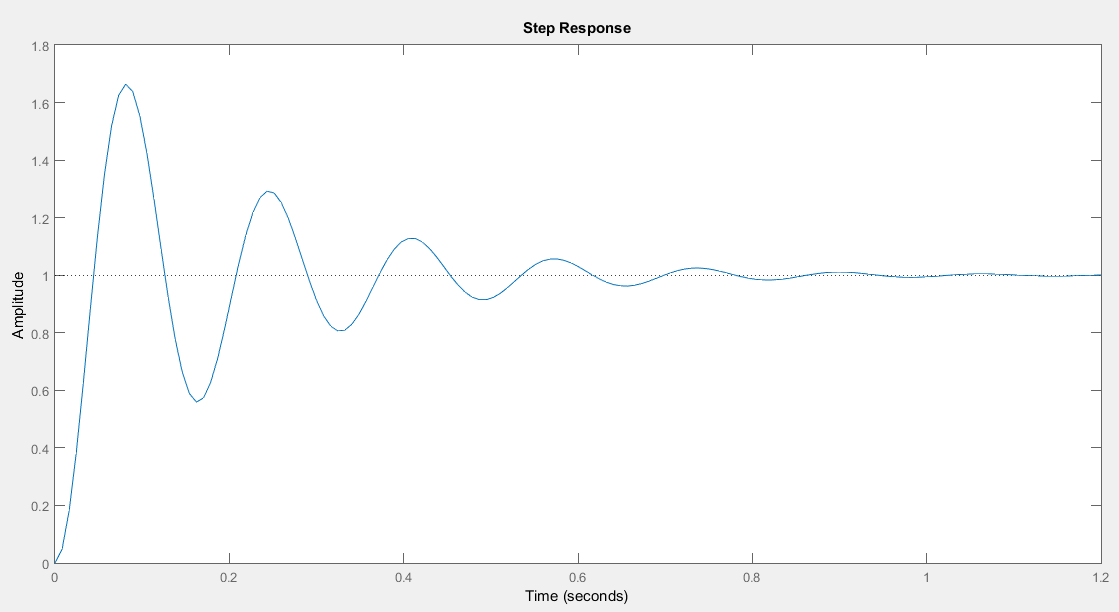
\includegraphics[width = 0.7\textwidth]{figure/plot_orde_dua.png}
    \caption{Plot respon sistem orde dua}
\end{figure}

\subsection{Analisis Grafik Respon Sistem Orde Dua}

\begin{figure}[H]
    \centering
    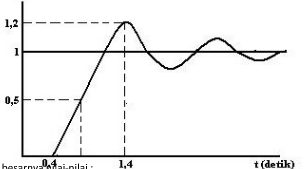
\includegraphics{figure/soal_5.png}
    \caption{Grafik Respon Sistem}
    \label{grafik_respon_sistem}
\end{figure}

Dari grafik diatas dapat dianalisis parameter sebagai berikut,

\begin{itemize}
    \item nisbah redaman ($\xi$)
    \item waktu puncak (peak time)
    \item waktu bangkit (rise time)
    \item waktu endap (settling time)
    \item waktu tunda (delay time)
\end{itemize}

\subsubsection{Nisbah Redaman}

Nisbah redaman dapat dicari dengan persamaan berikut,

\begin{equation}
    \begin{split}
        \%MP &= \exp{-\frac{\pi\xi}{\sqrt{1 - \xi^2}}}*100 \\[5pt]
        ln{[0.2]} &= \ln{[\exp{-\frac{\pi\xi}{\sqrt{1 - \xi^2}}}]} \\[5pt]
        1.61 &= \frac{\pi\xi}{\sqrt{1-\xi^2}} \\[5pt]
        \xi &= 0.46
    \end{split}
\end{equation}

\subsubsection{Waktu Puncak}

Nilai waktu puncak sudah tertampil di grafik sistem yaitu, $T_p = 1.4$ detik.
Dari waktu puncak, dapat dicari nilai $\omega_n$ sebagai berikut,

\begin{equation}
    \begin{split}
        T_p &= \frac{pi}{\omega_n\sqrt{1-\xi^2}} \Rightarrow \omega_n = \frac{\pi}{T_p\sqrt{1-\xi^2}} \\[5pt]
        \omega_n &= \frac{\pi}{1.4\sqrt{1-0.46^2}} \Rightarrow \omega_n = 2.53
    \end{split}
\end{equation}

\subsubsection{Waktu Bangkit}

Waktu bangkit dapat dihitung dengan persamaan berikut,

\begin{equation}
    \begin{split}
        T_r &= \frac{1}{\omega_n\sqrt{1-\xi^2}}[\pi-\arctan\frac{\sqrt{1-\xi^2}}{\xi}] \\[5pt]
        T_r &= \frac{1}{[2.53]\sqrt{1-0.46^2}}[\pi-\arctan\frac{\sqrt{1-0.46^2}}{0.46}] \\[5pt]
        T_r &= 1.39 \text{ detik} 
    \end{split}
\end{equation}

\subsubsection{Waktu Endap}

Waktu endap dapat dicari setelah menemukan nilai time constant, persamaan untuk mencari nilai time constant dan nilai waktu endap sebagai berikut,

\begin{equation}
    \begin{split}
        \tau &= \frac{1}{\omega_n\xi} \\[5pt]
        \tau &= \frac{1}{2.53[0.46]} \\[5pt]
        \tau &= 0.8593
    \end{split}
\end{equation}

\begin{equation}
    \begin{split}
        T_s(\pm5\%) &= 3\tau \Rightarrow T_s(\pm5\%) = 3[0.2] = 2.58 \text{ detik} \\[5pt]
        T_s(\pm2\%) &= 4\tau \Rightarrow T_s(\pm5\%) = 4[0.2] = 3.44 \text{ detik}\\[5pt]
        T_s(\pm0.5\%) &= 5\tau \Rightarrow T_s(\pm5\%) = 5[0.2] = 4.30 \text{ detik}
    \end{split}
\end{equation}

\subsubsection{Waktu Tunda}

Waktu tunda dapat dicari dengan persamaan sebagai berikut,

\begin{equation}
    \begin{split}
        T_d = 0.742\tau \Rightarrow T_d = 0.742[0.8593] = 0.6376 \text{ detik}
    \end{split}
\end{equation}

\end{document}